
\documentclass{article}

\usepackage[utf8]{inputenc} 
\usepackage{lmodern}
\usepackage{lipsum}
\usepackage[margin=1 in,left=1.5in,includefoot]{geometry}
\usepackage{graphicx}
\usepackage{float}
\usepackage[hidelinks]{hyperref}
\usepackage{braket}

\usepackage{amsmath}



 %Allows for clickable references

%Header and Footer Stuff
\usepackage{fancyhdr}
\pagestyle{fancy}
\fancyhead{}
\fancyfoot{}
\fancyfoot[R]{ \thepage\ }
\renewcommand{\headrulewidth}{0pt}
\renewcommand{\footrulewidth}{0pt}
%

%Math part

\usepackage{amsfonts}
\usepackage{amsmath}




\begin{document}

\begin{titlepage}
	\begin{center}
	\line(1,0){330} \\
	\vspace{.75 cm}
	\huge{\bfseries D-Wave-Computer}\\
	\vspace{.25 cm}
	\line(1,0){330} \\
	\vspace{1.5 cm}
	\textsc{\LARGE Hochschule M\"unchen}\\
	%Figure
	%\begin{figure}[H]
	%	\centering
%		\includegraphics[height=0 cm] {path}
	%	\caption[Optional caption]{Real, local caption}
	%	\label{fig:Stefan}
	%\end{figure}
	\vspace{10 cm}
	\end{center}
	\begin{flushright}
	\textsc{\large Stefan Ronczka\\26.12.2016}
	\end{flushright}
\end{titlepage}

\tableofcontents
\thispagestyle{empty}
\cleardoublepage

\setcounter{page}{1}
\section{Einleitung}\label{sec:intro}

Um zu verstehen was der D-Wave Computer eigentlich tut und kann, sollte man sich allgemein klar machen, welche Vorteile Quanten Computer haben.
Dazu werden in dieser Arbeit die Grundgedanken entsprechend erläutert, wobei mehr der mathematische Teil im Vordergrund steht. Da der D-Wave, diese Physikalisch umsetzt, werden auch hier ein paar der Grundbausteine erklärt.
Um Abschließend nachvollziehen zu können, wie diese Technik auf mehrere Problem anwendbar ist, wird auch die Programmierung, das Mapping auf Quantenprobleme, eingegangen.

\section{Das Lichtschalterspiel}\label{sec:historyDWave}

Um nun in das Thema einzutauchen, wird nun anhand des Lichtschalter Spiels
die Allgemeine Problematik gezeigt.	

\begin{figure}[H]
		\centering
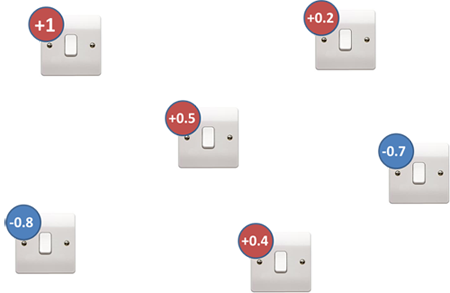
\includegraphics[scale=	1.5]{C:/Users/Stefan/Documents/GitHub/Seminararbeit/QuanteninfoBilder/tut-intro-lightswitch1.png}

\end{figure}

\
\
\flushleft
Für das Spiel gelten folgende Regeln:


\begin{itemize}


\item die Nummerierung der Schalter nennen sich Bias sie können den Wert einer beliebigen Zahl besitzen.

\item ein Schalter kann jeweils nur den Zustand 1 oder -1 besitzen, also an oder aus sein.

\item Gesucht ist nun die minimale Summe der Schalter anhand vom jeweiligen Zustand und Bias.


\end{itemize}


Mathematisch zusammen erfasst ergibt sich dieser Ausdruck.

\begin{equation}
E(s) = \sum_{i} h_{i}s_{i}
\label{schalterspiel1}
\end{equation}

wobei $s_{i}$ der Zustand von Schalter $i$ ist 
und $h_{i}$ dessen Bias

Wenn man ein bisschen überlegt findet sich die Minimale Lösung dieses Problems leicht. Denn das Minimum ist gerade dann der Fall wenn man 
die Vorzeichen des Bias negiert, also die Schalter mit positiven Bias auf "aus" und die mit negativen Bias auf "an" stellt.

\newpage

Fügt man diesem Problem eine weitere Regel, die Möglichkeit der Verknüpfung zweier Schalter, hinzu, lässt es sich nicht mehr ganz so einfach Lösen.


\begin{figure}[H]
		\centering
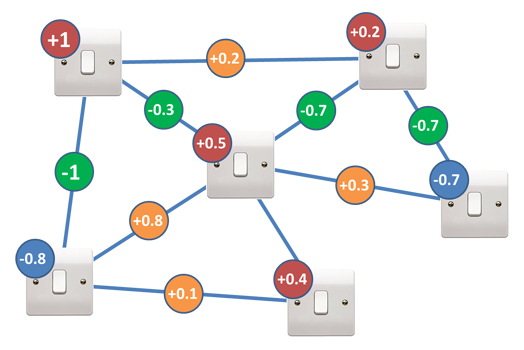
\includegraphics[scale=	1.5]{C:/Users/Stefan/Documents/GitHub/Seminararbeit/QuanteninfoBilder/tut-intro-lightswitcheshandj.png}


\end{figure}


Dazu werden die Verbindung zweier Schalter durch Multiplikation deren
Zustände realisiert. Zusätzlich wird ein gemeinsamer Bias zugeordnet wird.

\begin{equation}
E(s) = \sum_{i} h_{i}s_{i} + \sum_{i,j} J_{i,j} s_{i} s_{j}
\label{schalterspiel2}
\end{equation}


Wobei hier $_{i,j}$ der oben erwähnte gemeinsame Bias ist.
$s_{i}$ und $_{j}$ sind die Zustände der Verbundenen Schalter.
\newline


Wenn nun eine komplexe Schaltung, wie in der obigen Abbildung, gegeben ist,
in der alle Schalter einen oder mehrere Nachbarschalter haben, ist es schwer die Lösung zu bekommen.
Durch Aufprobieren sieht man sehr schnell, dass man mit dem Ansatz der leichteren Formel aus (\ref{schalterspiel1}) hier auch nicht weit kommt. 
Das ist auch kein Wunder, denn es gibt jetzt zwischen 2 Schaltern 
bis zu $2^2 = 4$ Möglichkeiten nämlich [An An] [An Aus][Aus An] und [Aus Aus].
Betrachtet man nun den schlimmsten Fall, das jeder Schalter mit jedem verbunden ist, steigt die Anzahl der möglichen Kombinationen exponentiell $2^n$.
\newline
\newline
In diesen Beispielen sind die Auswirkungen auf größere Schaltungen sichtbar.

\begin{align*}
2^2 = 4\\
2^{10} = 1024\\
2^{100} = 1.267.650.600.228.229.401.496.703.205.376\\
\end{align*}


\newpage

Wie also soll man das Spiel gewinnen? Selbst mithilfe von Super Computer ist
laut den D-Wave Wissenschaftlern schwierig(wenn nicht unmöglich) für System der Größe von 500 Schaltern zu berechnen, da nicht genug Zeit im Universum ist, um alle Kombinationen auszuprobieren. Die Lösung diese Problems ist der D-Wave Quantencomputer. Aufgrund der Quantenmechanik ist es möglich die Zustände aus Superposition von allen Zuständen zu beschreiben. Dazu werden die 
normalen Bits durch sogenannte Qubits ausgetauscht. Der D-Wave Computer nimmt sich diese Superpostion noch ohne Bias. Man passt nun der 
Quanten Computer langsam an, um den Superposition Effekt zu deaktivieren. Gleichzeitig werden die Bias J und h langsam aktiviert. Nun wirkt die Quantenmechanik auf die Schalter und hilft ihnen den Zustand für die minimale Summe zu finden. Nachdem dies geschehen ist, befinden sich die Schalter in einem Klassischen Zustand. So wie die Schalter nun stehen, ist die Kombination für das globale Minimum.

\section{Die Alogrithmen}\label{sec:baseAlgo}
Damit ist natürlich noch nicht beantwortet was hinter dem Vorgehen des D-Wave Computers steckt.
Um dies näher zu bringen, wird nun in diesem Teil 
die Optimierungs Strategie des D-Wave gezeigt.
Der D-Wave konzipiert auf den fundamentalen Prinzipien der Natur. Dort gilt für alle physikalischen Systeme, dass sie dazu neigen ihre freie Energie zu minimieren. Genau diese Eigenschaft wird in klassischen 
Systemen meist mit "Annealing" verbunden.
Annealing bedeutet soviel wie abkühlen, genauer ist mit "thermal Annealing" ein Vorgang gemeint, der aus der Werkstoffkunde kommt. Hier wird das Metall ,nachdem  erhitzen, langsam abgekühlt. Dies Sorgt dafür, dass die Atome die Zeit haben sich zu ordnen und Kristalle zu bilden.%def wiki themal annealing 
Hierbei wird das Metall von Unreinheiten (den großen Energie) befreit.
Es wird also wie oben bereits gesagt diese Energie minimiert. Dies geschieht, aber eben nur wenn man dem System genügend Zeit lässt. Es gibt nun mehrerer Annealing Algorithmen, wobei sich auf die von D-Wave genutzten "adiabatic quantum Computation" beschränkt wird, da es von hier aus leichter ist die Verbindung zum D-wave klar zumachen. Das erste was einem dabei auffällt ist der Begriff "adiabatic" oder zu Deutsch adiabatisch. Um diesen Begriff zu erklären werden allerdings noch ein paar Quantenmechanische Formeln benötigt. Zunächst die Schrödinger Gleichung,welche die Dynamik eines Quantenmechanischen Zustandes beschreibt.
\begin{equation}
i\hbar\frac{ \partial}{ \partial t} \ket{\psi (t)} = \hat{H} \ket{\psi (t)}
\end{equation}
\newline
$\hat{H}$ ist hierbei der Hamiltonoperator, er steht für die gesamte Energie des Systems.
$\hbar$ ist das Plancksche Wirkungsquantum und
$\frac{ \partial}{ \partial t}$ die Ableitung nach der Zeit
Dabei ist $\ket{\psi (t)}$ ist der Zustandsvektor in einem Hilbertraum.


Durch einsetzten 




Man kann sich dies auch so vorstellen ,dass man eine Landschaft aus dem Energiepotenzial der 

Auch in Quanten Systemen ist dies so, wobei sich gezeigt hat, dass der Vorgang hier noch 
im Gegensatz zu obigen Beispiel beschleunigt wird.



Der D-Wave ist so entworfen worden das man das man eigentlich jeden Quantum Anne


Quantum Annealing ist eine Methode zur Bestimmung des lokalen Optimums bei vielen Unabhängigen in einem Funktion. Genauer handelt es sich um eine Metaheuristik, die also theoretisch auf auf beliebig viele Problemstellungen angewandt werden kann, wenn sie für das Problem implementiert wird.

Speziell verwendet D Wave Computer Adiabatische Quanten Berechnungen,
da ein allgemeiner 
 




\subsection{Aufbau}\label{sec:funktion}\cite{ref:one}

\subsection{Schwierige Probleme lösen mit Physik}\label{sec:historyAlgo}
\subsection{Der Algorithmus}\label{sec:algo}
\section{Struktur der Software}\label{sec:software}
\section{Anwendung auf komplexe Probleme}\label{sec:problems}

%References
\cleardoublepage
\bibliographystyle{plain}
\bibliography{/references/firstref.bib}





\end{document}